\documentclass[dvipdfmx, titlepage, 11pt]{jsarticle}
\usepackage{tikz}
\usetikzlibrary{patterns}
\usetikzlibrary{intersections,calc,arrows}
\usepackage[top=20truemm,bottom=20truemm,left=15truemm,right=15truemm]{geometry}
\usepackage{enumerate}
\usepackage{multicol}
\usepackage{diagbox}
\usepackage{graphicx}

\makeatletter
\newcommand{\overarc}[1]{
  \setbox0\hbox{#1}%
  \ifdim\wd0<1em%
    \stackrel{\frown}{#1}%
  \else\ifdim\wd0<1.75em%
    \stackrel{\rotatebox{90}{\big)}}{#1}%
  \else\ifdim\wd0<2.5em%
    \stackrel{\rotatebox{90}{\Big)}}{#1}%
  \else\ifdim\wd0<3.25em%
    \stackrel{\rotatebox{90}{\bigg)}}{#1}%
  \else%
    \stackrel{%
      \rotatebox[origin=c]{90}{\mbox{%
        $\left.\vphantom{\rotatebox[origin=c]{90}{#1}}\right)$%
      }}%
    }{#1}%
  \fi\fi\fi\fi%
}
\makeatother



\title{\Huge 数学}
\author{\LARGE 試験時間 : 50分}
\date{\LARGE 平成28年度筑波大附属高校\\[3cm] 大問は \fbox{\Large {\bf 1}} から \fbox{\Large {\bf 5}} まであります\\[0.5cm] 解答は解答用紙に記入して下さい}
\begin{document}
\maketitle

\newpage
\thispagestyle{empty}
 
\newpage

\newpage
\thispagestyle{empty}
 
\newpage

\setcounter{page}{1}
\noindent \fbox{\LARGE {\bf 1}}\hspace{10pt} 次の\textcircled{\scriptsize 1} 〜 \textcircled{\scriptsize 4}の \fbox{ \hspace{10pt} } にあてはまる数を求めなさい.
\begin{enumerate}[(1)]
\item $x =\sqrt{3} + \sqrt{2}$,\ \ $\displaystyle y = \frac{\sqrt{3}-\sqrt{2}}{2}$ のとき, $(x+y)^{2}-y(2x+5y)$ の値は \fbox{\hspace{5pt} \textcircled{\scriptsize 1}\hspace{5pt} } である.\\[5cm]
\item 4個の数字1,\ \ ,2,\ \ 3,\ \ 4が, はじめこの順に並んでいる. 1回の操作で, でたらめに2つの数字の位置を入れかえる. この操作を2回続けて行ったとき, 1が左端にある確率は \fbox{\hspace{5pt} \textcircled{\scriptsize 2}\hspace{5pt} } である.
\newpage
\item 下の図1において, 5点A,\ \ B,\ \ C,\ \ D,\ \ Eは円周上の点であり, $\angle$CAD = $42^{\circ}$,\ \ $\overarc{\rm AB} = \overarc{\rm BC}$,\ \ $\overarc{\rm AE} = \overarc{\rm ED}$である.\\
  2直線BC,\ \ EDの交点をFとするとき, $\angle$CFD = \fbox{\hspace{5pt} \textcircled{\scriptsize 3}\hspace{5pt} } 度である.\\

  \begin{tikzpicture}

    \node at (-2.1, 2.3) {図1};
    \draw[name path = C] (0,0) circle[radius=2];

    \draw[name path = L] (135:2) node[left] {E} -- (5.7,1.2) node[right] {F} -- (270:2) node[below] {B};
    \path[name intersections = {of = C and L}];
    \draw (intersection-1)node[above right] {D} -- (212:2) node[left] {A}-- (intersection-3) node[below right] {C};
  \end{tikzpicture}

  \vspace{3cm}
  
\item 下の図2のように, すべての辺の長さが3cmの正四角すいO-ABCDがある. 辺OB, ODの中点をそれぞれP,\ \ Qとし, 3点A,\ \ P,\ \ Qを含む平面とOCとの交点をRとするとき,\ 線分ARの長さは \fbox{\hspace{5pt} \textcircled{\scriptsize 4}\hspace{5pt} } cmである.

  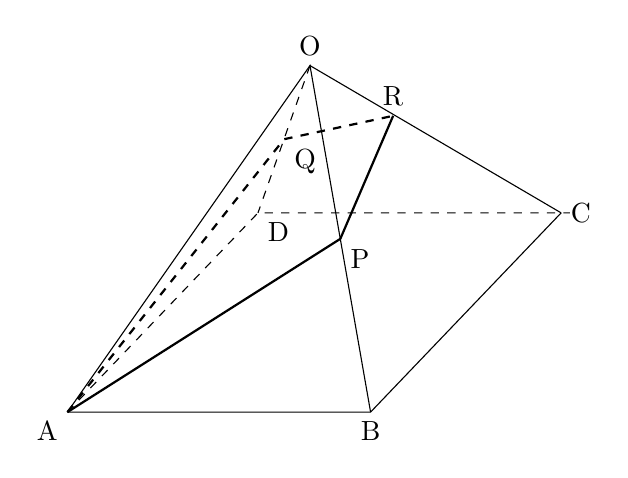
\begin{tikzpicture}[scale=1.1]
    \draw (0,0) node[below left] {A} -- (3.5,0) node[below] {B} -- (5.7, 2.3) node[right] {C};
    \draw[dashed] (0,0) -- (2.2,2.3) node[below right] {D} -- (5.8, 2.3);

    \coordinate (O) at (2.8, 4);
    \draw (0,0) -- (O) node[above] {O} -- (3.5,0);
    \draw (O) -- (5.7,2.3);
    \draw[dashed] (O)--(2.2,2.3);
    \coordinate (P) at (3.15, 2);
    \coordinate (R) at (3.76, 3.42);
    \coordinate (Q) at (2.5, 3.15);

    \draw[thick] (0,0)--(P) node[below right] {P}--(R);
    \draw[thick, dashed] (0,0)--(Q) node[below right] {Q} --(R) node[above] {R};
  \end{tikzpicture}
\end{enumerate}

\newpage

\noindent \fbox{\LARGE {\bf 2}}\hspace{10pt} 40人の生徒に100点満点の数学の試験を実施した. 下の度数分布表はその結果をまとめたものであるが, ?となっている欄の人数はわからなくなっている. 40人の得点はすべての整数値であり, 中央値は59.5点で, 満点の生徒はいなかった.\\
このとき, 次の\textcircled{\scriptsize 5}の \fbox{ \hspace{10pt} } にあてはまる数を求め, \textcircled{\scriptsize 6}の解答欄には求め方と人数を書きなさい.\\

\begin{tabular}{|c|c|c|} \hline
  階 級 &階級値(点) & 度数(人)\\ \hline
  0点以上〜10点未満&5&0\\ \hline
  10 〜 20 &15&0\\ \hline
  20 〜 30 &25&1\\ \hline
  30 〜 40 &35&4\\ \hline
  40 〜 50 &45&7\\ \hline
  50 〜 60 &55&?\\ \hline
  60 〜 70 &65&7\\ \hline
  70 〜 80 &75&?\\ \hline
  80 〜 90 &85&?\\ \hline
  90 〜 100 &95&7 \\ \hline
  合計&\diagbox[width=2.5cm, height=0.55cm]{}{}&40\\ \hline
\end{tabular}

\begin{enumerate}[(1)]
\item 50点以上60点未満の生徒の人数は, \fbox{\hspace{5pt} \textcircled{\scriptsize 5}\hspace{5pt} } 人である.\\[2cm]
\item この度数分布表を利用して40人の得点の平均値を求めた結果, 平均値は整数値であった. このとき, 70点以上80点未満の生徒の人数は何人であるか. \textcircled{\scriptsize 6} の解答欄に求め方と人数を書きなさい.
\end{enumerate}

\newpage
\noindent \fbox{\LARGE {\bf 3}}\hspace{10pt} ある自動車の燃料タンクにガソリンを最大限入れ, 燃料がなくなるまで走らせる. \\
(ア) 〜 (ウ)のことが分かっているとき, 次の\textcircled{\scriptsize 7} 〜 \textcircled{\scriptsize 9}の \fbox{ \hspace{10pt} } にあてはまる数または式を求めなさい.

\begin{center}
  \begin{tikzpicture}
    \draw[dotted] (-0.3,-0.9) rectangle (13.5,0.9);
    \draw (0,0.5) node[right] {(ア) 時速30kmで走らせると, 走行時間は11時間である.};
    \draw (0,0) node[right] {(イ) 速度の増加に応じて, 走行時間は一定の割合で減少する.};
    \draw (0,-0.5) node[right] {(ウ) 時速40kmで走らせる場合と, 時速100kmで走らせる場合の走行距離は等しい.};
  \end{tikzpicture}
\end{center}

\begin{enumerate}[(1)]
\item 時速$x$kmで走らせたところ, 走行時間は$y$時間であった. $y$を$x$の式で表すと, $y=$ \fbox{\hspace{5pt} \textcircled{\scriptsize 7}\hspace{5pt} } である.\\[3cm]
\item 時速$a$kmで走らせたところ, 走行距離は490kmであった. このとき, $a=$ \fbox{\hspace{5pt} \textcircled{\scriptsize 8}\hspace{5pt} } である.\\[3cm]
\item 時速70kmで$b$時間走らせた後, 時速98kmで$c$時間走らせたところ, 走行距離は462kmであった. 走行時間の合計$(b+c)$は, \fbox{\hspace{5pt} \textcircled{\scriptsize 9}\hspace{5pt} } 時間である.
\end{enumerate}
\newpage

\begin{minipage}{0.6\hsize}
  \noindent \fbox{\LARGE {\bf 4}}\hspace{10pt} AD//BC,\ \ AD=4cm,\ \ $\angle$Aが鋭角である台形ABCDの辺上を動く2点P,\ \ Qがある.\\
  点PはAを出発し, 一定の速さで辺AD上をDまで動き, 点QはPと同時にAを出発し, 一定の速さで辺AB, 辺BC上をCまで動く\\
  PがDに到達すると同時に, QはCに到達した.\\
  台形ABCDを線分PQで2つの図形にわけるとき, Aを含む図形をFとする. 2点P,\ \ QがAを出発してから$x$秒後の図形Fの面積を$y$ cm${}^{2}$とすると,\ \ $x$と$y$の関係を表すグラフは右図のようになった. \\
  このとき, 次の\textcircled{\scriptsize 10} 〜 \textcircled{\scriptsize 12} の \fbox{ \hspace{10pt} } のあてはまる数を求めなさい.\\[2cm]
\end{minipage}
\begin{minipage}{0.35\hsize}
  \begin{center}
    \begin{tikzpicture}
      \draw(-0.5,0)--(3.7,0) node[right] {$x$};
      \draw(0,-0.5)--(0,7.5) node[above] {$y$};
      \draw[thick,dotted] (1.5,0) node[below] {4}--(1.5,1.5)--(0,1.5)node[left] {4};
      \draw[thick,dotted] (3,0)node[below] {8} -- (3,6.75) -- (0,6.75) node[left] {18};
      \draw[thick] (0,0) parabola (1.5,1.5)--(3,6.75);
      \node at (-0.25,-0.25) {O};
    \end{tikzpicture}
  \end{center}
\end{minipage}
\newpage

\begin{enumerate}[(1)]
\item 辺BCの長さは \fbox{\hspace{5pt} \textcircled{\scriptsize 10}\hspace{5pt} } cmである.\\[4cm]
\item 辺CDの長さは \fbox{\hspace{5pt} \textcircled{\scriptsize 11}\hspace{5pt} } cmである.\\[4cm]
\item PQ=5cmとなるのでは,\ \ 2点P,\ \ QがAを出発してから \fbox{\hspace{5pt} \textcircled{\scriptsize 12}\hspace{5pt} } 秒後である.
\end{enumerate}

\newpage

\noindent \fbox{\LARGE {\bf 5}}\hspace{10pt} 下図のように, AB=8cm,\ \ BC=16cm,\ \ CA=12cmの$\triangle$ABCにおいて, 辺BCを四等分する点をD,\ \ E,\ \ Fとする.\\
$\angle$Bの二等分線とAD,\ \ AE,\ \ AF,\ \ ACとの交点をそれぞれP,\ \ Q,\ \ R,\ \ Sとするとき, 次の\textcircled{\scriptsize 13} 〜 \textcircled{\scriptsize 15}の \fbox{ \hspace{10pt} }にあてはまる数または式を求めなさい.

\begin{center}
  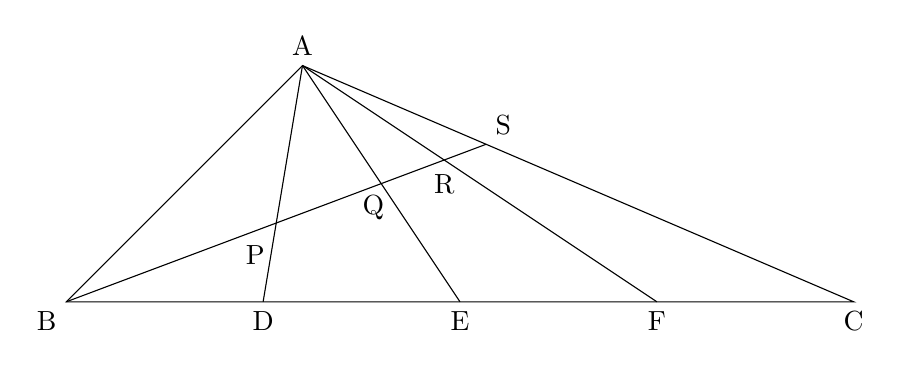
\begin{tikzpicture}
    \coordinate (A) at (3,3);
    \coordinate (B) at (0,0);
    \coordinate (C) at (10,0);
    \coordinate (D) at (2.5, 0);
    \coordinate (E) at (5,0);
    \coordinate (F) at (7.5,0);

    \draw (A)node[above] {A}--(B)node[below left] {B}--(C)node[below] {C}--cycle;
    \draw (A)--(D)node[below] {D};
    \draw (A)--(E)node[below] {E};
    \draw (A)--(F) node[below] {F};

    \coordinate (S) at (5.33, 2);
    \draw (B)--(S) node[above right] {S};
    \node at (2.4,0.6) {P};
    \node at (3.9,1.2) {Q};
    \node at (4.8,1.5) {R};
  \end{tikzpicture}
\end{center}

\vspace{2cm}

\begin{enumerate}[(1)]
\item 線分ADの長さは, \fbox{\hspace{5pt} \textcircled{\scriptsize 13} \hspace{5pt} } cmである.\\[3cm]
\item 線分PQの長さは, \fbox{\hspace{5pt} \textcircled{\scriptsize 14} \hspace{5pt} } cmである.\\[3cm]
\item 線分PQ,\ \ QR,\ \ RSの長さの比をもっとも簡単な整数の比で表すと, PQ : QR : RS = \fbox{\hspace{5pt} \textcircled{\scriptsize 15}\hspace{5pt} } である.
\end{enumerate}
\newpage
\thispagestyle{empty}
 
\newpage

\newpage
\thispagestyle{empty}
 
\end{document}